\documentclass[a4paper]{article}
\usepackage{fancyhdr}
\usepackage[backend=bibtex, style=authoryear, uniquename=init, giveninits=true, maxbibnames=3, minbibnames=2]{biblatex} 
\usepackage{lastpage}
\usepackage[utf8]{inputenc}
\usepackage[official]{eurosym}
\usepackage[right=30mm,left=30mm,top=30mm,bottom=30mm]{geometry} 
\usepackage{graphicx} % support the \includegraphics command and options
\usepackage{amsmath}
\usepackage{amssymb}
\usepackage{adjustbox}
\usepackage{mathtools}
\usepackage{subcaption}
\usepackage{centernot}
\usepackage[parfill]{parskip} % Activate to begin paragraphs with an empty line rather than an indent
\usepackage{booktabs} % for much better looking tables
\usepackage{array} % for better arrays (eg matrices) in maths
\usepackage{paralist}% very flexible & customisable lists (eg. enumerate/itemize, etc.)
\usepackage{verbatim} % adds environment for commenting out blocks of text & for better verbatim
\usepackage[table,xcdraw]{xcolor}
\usepackage{perpage}
\usepackage{hyperref}
\usepackage[perpage,symbol*]{footmisc}
\usepackage{chngcntr}
\usepackage{amsthm}
\usepackage{makecell}
\usepackage{csquotes}
\usepackage[nottoc,numbib]{tocbibind}
\counterwithin{figure}{section}
\counterwithin{equation}{section}
\counterwithin{table}{section}
\allowdisplaybreaks
\linespread{1.2}
\pagenumbering{arabic}
\title{Who smokes?}
\author{Samuel Hashem Zehi}
\date{Student ID: 1591277}
\theoremstyle{definition}
\newtheorem{definition}{Definition}[section]
\newtheorem{concept}{Concept}
\newtheorem{lemma}{Lemma}[section]
\newtheorem{rmrk}{Remark}[section]
\newtheorem{note}{Note}[section]
\renewcommand{\thefootnote}{\fnsymbol{footnote}}
\newcommand*\diff{\mathop{}\!\mathrm{d}} %Integral d 
\newcommand{\mbg}{\overset{!}{>}} %must be greater
\newcommand{\mbeq}{\overset{!}{=}} %must be equal
\newcommand{\mnbq}{\overset{!}{\neq}}  %must be unequal
\newcommand{\df}{\partial} %partial derivatives
\newcommand{\fr}{\frac} %fractions
\DeclareMathOperator*{\argmax}{argmax} %argmax proper
\DeclareMathOperator*{\argmin}{argmin} %argmin proper
\newcommand{\uline}{\underline} %underline
\newcommand{\bpm}{\begin{pmatrix}} %matrix shortcuts 4x
\newcommand{\epm}{\end{pmatrix}}
\newcommand{\bbm}{\begin{bmatrix}}
\newcommand{\ebm}{\end{bmatrix}}
\newcommand{\beq}{\begin{equation}} %equation 
\newcommand{\eeq}{\end{equation}}
\newcommand{\beqq}{\begin{equation*}} %unnumbered equation 
\newcommand{\eeqq}{\end{equation*}}
\newcommand{\hbeta}{\hat{\beta}} %estimator for beta
\newcommand{\e}{\epsilon}
\newcommand{\sbdist}{\Sigma_{\sqrt{n}(\hat{\beta}-\beta)}} %Covarianz Matrix for distribution 
\newcommand{\convdist}{\overset{d}{\longrightarrow}} %convergence in distribution
\newcommand{\convprob}{\overset{p}{\longrightarrow}} %convergence in probability
\newcommand{\asymdist}{\overset{a}{\sim}} %asymptotically distributed
\newcommand{\x}{\times} %matrix and vector dimension notation, e.g. x is a k \x 1 vector of regressors
\DeclareCiteCommand{\citeauthorfirstlast}
  {\boolfalse{citetracker}%
   \boolfalse{pagetracker}%
   \DeclareNameAlias{labelname}{first-last}%
   \usebibmacro{prenote}}
  {\ifciteindex
     {\indexnames{labelname}}
     {}%
   \printnames{labelname}}
  {\multicitedelim}
  {\usebibmacro{postnote}}

\DeclareCiteCommand{\citeauthorlastfirst}
  {\boolfalse{citetracker}%
   \boolfalse{pagetracker}%
   \DeclareNameAlias{labelname}{last-first}%
   \usebibmacro{prenote}}
  {\ifciteindex
     {\indexnames{labelname}}
     {}%
   \printnames{labelname}}
  {\multicitedelim}
  {\usebibmacro{postnote}}
\hypersetup{colorlinks, citecolor=black, filecolor=black, linkcolor=black, urlcolor=black} %%for links to not be visible
\bibliography{ideas}
\begin{document}
\begin{titlepage}
\vspace*{0.8cm}
\begin{figure}[!h]
\centering

\includegraphics[width = 0.5\textwidth]{Uni_Logo_2016.png}
\end{figure}
\begin{center}

\vspace*{1,2cm}

\huge {\bfseries Search Interest for Gold Prices and Realized Gold Prices}\\[1.8cm]

\Large {Macroeconometrics}\\[1cm]
\end{center}
\vspace{2cm}

\noindent \textbf{Supervisor:}\\
Univ.-Prof.\ Dipl.-Ing.\ Dr.\ Robert Kunst\\

\vspace{1cm}

\noindent \textbf{Authors:}\\
Hashem Zehi, Samuel (Student ID 12012285) \\
Hochholzer, Matthias (Student ID 11724853) \\

\vspace{1cm}

\noindent Master of Science Economics (M.Sc.)\\

\vspace{1cm}

\noindent Vienna, \today

\setcounter{page}{0}\clearpage
\end{titlepage}
\newpage
\tableofcontents
\newpage
\section{Introduction}
This project investigates the relationship between the realized price of gold and a standardized index measuring the relative online search interest for gold prices. More specifically, can search interest help improve prediction of one-period ahead gold prices. Due to the technological advances in the financial industry nowadays more and more algorithms work based on internet sentiment in order to buy and sell financial products. One possible measure for such automated algorithms is using data provided by companies like Google or Microsoft. Large spikes in search interest may trigger such algorithms. As financial news outlets like Bloomberg or the Financial Times write articles on price changes more and more people will look up prices of goods and commodities, again triggering the algorithms, resulting in a feedback loop. 

This paper is structured as follows. First we explain the data collection process then do some exploratory data analysis. Then we attempt to find the best prediction model for gold prices. Afterwards we model the gold price and the relative search interest jointly. Lastly we give some closing remarks on our results and issues with modeling and data.
\section{Data}
The data used in this project comes from two sources. Firstly the gold price search interest is provided to the public by \citeauthor{Google.2021} (\citeyear{Google.2021}). This data is standardize to a range from zero to 100 over the entire time range. 100 represents the point in time with the highest search interest and zero either no interest at all or simply not enough data for this specific point in time. 50 then simply means that the popularity is at 50\% of the peak value. Due to the ability to collect a wide range of data on the users of the website Google removes datapoints where the same user looked the term up multiple times within a short period of time. Furthermore, regional differences  are accounted for due to the data only being relative search interest, thus regions with larger populations and particular search interests cannot skew the data. It is noteworthy that if the data is split up by regions India, one of the largest markets for gold, appears to have the highest relative search interest, with only countries like Oman, Pakistan, and Myanmar being close. For this analysis we focus on the worldwide interest in the search term \textquote{gold price} over the period 2004 until June 2021.

Secondly, the data on gold prices is provided by \citeauthor{ICEBenchmarkAdministrationLimited.} (\citeyear{ICEBenchmarkAdministrationLimited.}) and published for use by the Economic Research Division of the Federal Reserve Bank St.\ Louis and collected by the London Bullion Market Association. The price is set twice daily, in the morning and the afternoon, and measured in US dollars per troy ounce. For our analysis we use the afternoon price given two separate frequencies. When not modeling the data jointly we use a daily frequency as it allows us to make a more detailed analysis and gives a more accurate reflection of the volatility. It should be noted that there around 200 of the 5,300 observations contain \textquote{NA} values. As there appears to be not specific pattern such as for example no prices being reported on weekends, we have elected to replace these values with the price from the previous day.  

In the joint modeling we are constrained by the frequency with which Google makes search interest data available: monthly. Thus we use a monthly frequency for the realized prices as well, to be more precise we use the prices at the end of each month. 
\newpage
\section{Gold Price Modeling}
\subsection{Exploratory Analysis and Unit-Root Testing}
In this section look at the daily price of gold. We start by taking a unit-root test on the daily gold price. We have augmented Dickey-Fuller test with the following regression which is then estimated:
	\begin{align*}
	\Delta y_t = a_0 + \gamma \cdot y_{t-1} + a_2 \cdot t + \epsilon_{t}
	\end{align*}
The hypothesis are given by $\tau: \gamma = 0$, $\phi_3: \gamma = a_2 = 0$, and $\phi_2: a_0 = \gamma = a_2 = 0$. Thus we have three test-statistics. For all three test-statistics we fail to reject the null at the 10\% level. Together, this implies that given the data we cannot reject the hypothesis of a unit-root, neither can we reject the hypothesis of no time trend or no drift. Figure 3.1 shows how the daily gold price developed from early 2001 until mid 2021.
	\begin{figure}[!t]
	\centering
	\caption{Daily Gold Prices}
	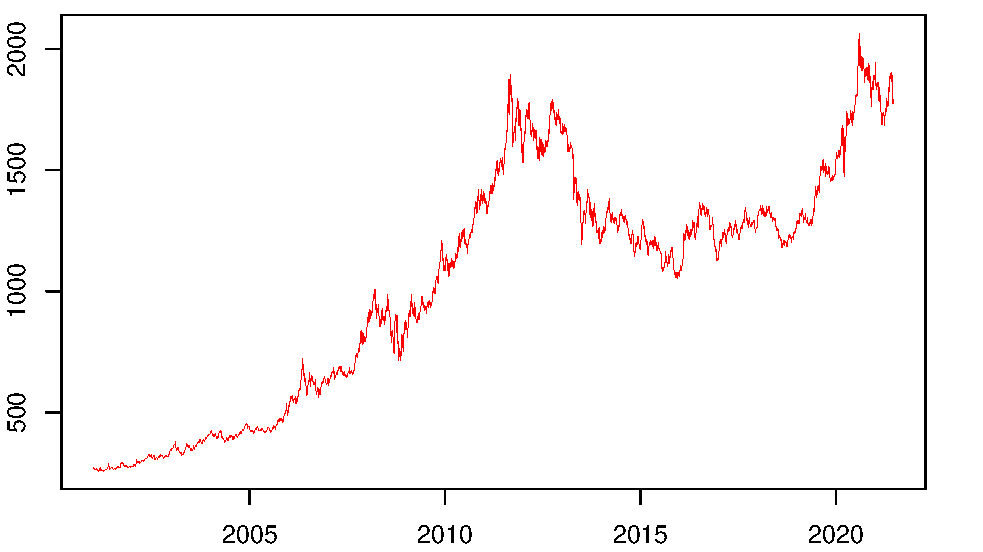
\includegraphics[width=0.90\textwidth]{goldPriceHF.pdf}
	\end{figure}

We can see three separate phases in the development of this variables. From the beginning until around 2012 we can observe an almost linear increase of the price peaking at almost USD 2,000, followed by around four years of linear decrease back to around USD 1,200. Then we again observe an increase until mid 2021 with a new peak at around USD 2,000. This leads to the question whether or not conventional wisdom on the stability of gold prices holds true in the modern world.

Now we consider the first-differenced gold prices.
	\begin{figure}[!t]
	\centering
	\caption{Daily Gold Prices (First-Differences)}
	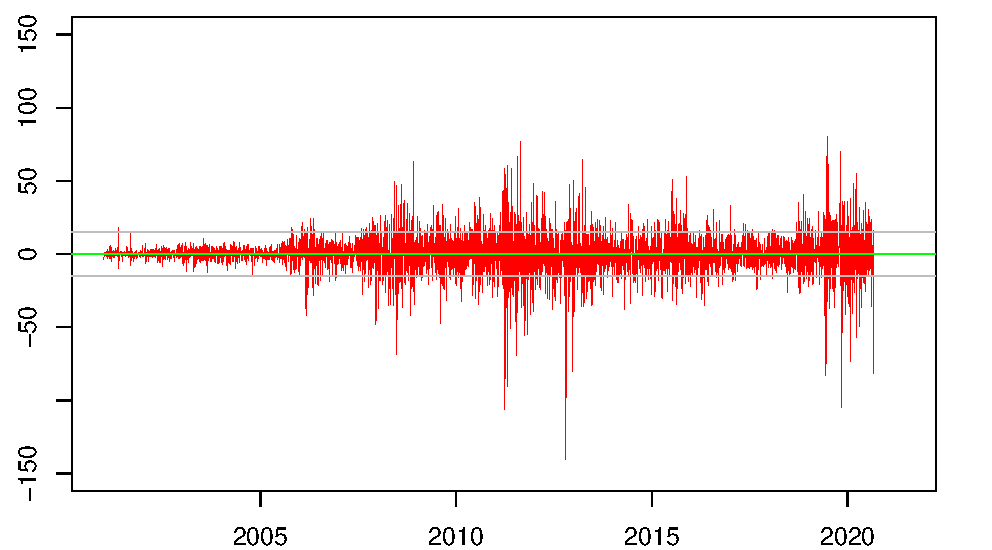
\includegraphics[width=0.90\textwidth]{goldFDHFalone.pdf}
	\end{figure}
At first glance they appear to be stationary around zero with phases of higher and lower volatility. The overall level of volatility appears to have increased starting from 2006 onward, as indicated by the gray lines. Before 2006 there were very few observations outside of the $\pm 15$ band, compared to this occurring very frequently afterwards. In order to illustrate the high frequency of data we chose very thin lines for Figure 3.2. It appears that there is some volatility clustering in the daily prices of gold. Four clusters appear very prominent, namely one at around 2007-2008, 2011, 2013, and 2019-2020. Every now and then there are very large outliers, one notable in 2013 with a day-on-day decrease by over USD 100.
\subsection{Best-Prediction Modeling}
Next we consider model selection for these high-frequency prices. We start by looking at the autocorrelation function (ACF) and partial autocorrelation function (PACF) of the first-differences. 
\begin{figure}[t]
     \centering
     \caption{Empirical (Partial) Autocorrelation Functions of the Gold Price FDs}
     \begin{subfigure}[t]{0.45\textwidth}
         \caption{ACF}        
         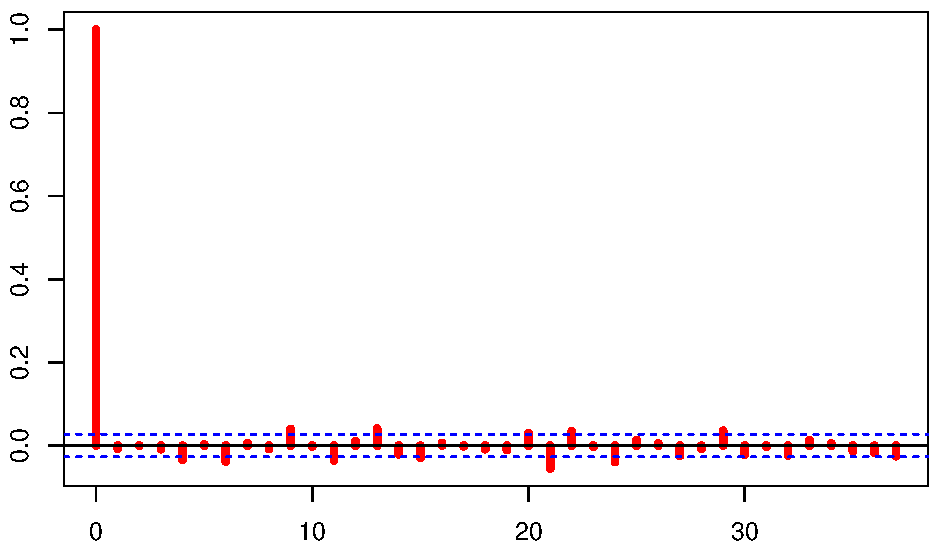
\includegraphics[width=\textwidth]{acfGOLDFD}
    \end{subfigure}
    \begin{subfigure}[t]{0.45\textwidth}
         \caption{PACF}
         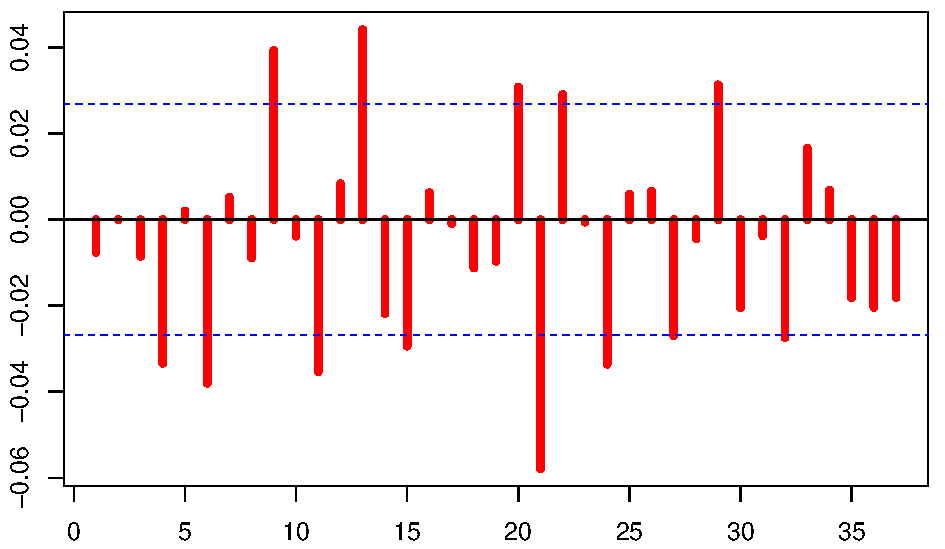
\includegraphics[width=\textwidth]{pacfGOLDFD}
    \end{subfigure}
\end{figure}

From Figure 3.3 we can see that there appears to be very little autocorrelation, with very few lags being non-zero. It seems like there is some wave pattern, albeit a very small one. The PACF indicates that most of the lags are - if significant - only slightly above or below the significance band. Some of the more notable lags are the 13$^{th}$ and the 21$^{st}$ ones, which seems significantly larger than zero in absolute value. 

In this section we use the AIC in order to determine the optimal lag order. As our data are of somewhat high frequency over a longer period of time, any concerns over the performance of the information criterion in small samples can be disregarded. When modeling prices we are often concerned with trying to predict prices, which justifies the choice of the AIC as it selects the best-forecasting model in large samples rather than leading to a consistent choice of lag orders. We estimate all ARIMA($p,d,q$) models within a range of $p$ and $q$ values and then choose the one with the lowest AIC value, where the criterion is defined as follows:
	\begin{align*}
	\text{AIC} = \log \hat\sigma^2 + 2 \frac{p+q+1}{2}.
	\end{align*}
The model selection works as follows. First the function finds the level of differencing which is needed to make the data stationary, then the function uses the AIC in order to determine the optimal lag order. For our data the function first selects $d=1$, i.e.\ the function selects the first-differences as the stationary variable. Then the function selects an ARIMA(0,1,0) model,  we have a model with no trend component but a drift component and $\hat\sigma^2 = 151.5$. The model can be described by the function
	\begin{align*}
	\Delta p^{HF}_{t} = \underset{[0.1685]}{0.2847} + \epsilon_{t},
	\end{align*}
where the standard error is in brackets. The AIC of this model is 41974.4. For comparison, if we used an MA(2) model on the first-differences we have an AIC value of 41979.1. Contrasting this frequency with the monthly gold prices we would select the following model:
	\begin{align*}
	\Delta p^{LF}_{t} = \underset{[3.6766]}{7.1279}  \underset{[0.0740]}{-0.1411}\epsilon_{t-1} + \epsilon_{t}.
	\end{align*}
It is noteworthy that the coefficients cannot be reasonably compared for both models due to the differences in the frequencies. Overall it appears to be the case that we cannot gain much information by looking at past price changes, but could rather always expect that the price changes from one day to another are constant over time and slightly positive. However, there are certain complications when looking at the volatility. 
\subsection{Volatility Analysis}
As mentioned in the exploratory analysis of the data it does not appear as if the autocovariance if constant over time. Thus it is a natural consequence to further look at ways of modeling the volatility. We do so by considering different extensions of ARCH models like the eGARCH. Again we use the AIC to evaluate the relative model performance against other specifications. We have the following four models. First we have the ARCH model estimated by
	\begin{equation}\tag{ARCH}
	\mathbb E(\epsilon_t^2 \mid \mathcal{I}_{t-1})= \sigma_t^2 = 117.24 + 0.27 \epsilon_{t-1}^2.	
	\end{equation}
Now we have the GARCH estimated by
	\begin{equation}\tag{GARCH}
	\mathbb E(\epsilon_t^2 \mid \mathcal{I}_{t-1})= \sigma_t^2 = 0.10 + 0.06 \epsilon_{t-1}^2 + 0.94 \sigma_{t-1}^2.
	\end{equation}
The third model is the iGARCH which is estimated as
	\begin{equation}\tag{iGARCH}
	\mathbb E(\epsilon_t^2 \mid \mathcal{I}_{t-1})= \sigma_t^2 = 0.13 + 0.06 \epsilon_{t-1}^2 + 0.94 \sigma_{t-1}^2.	
	\end{equation}
And lastly we have the eGARCH model by \citeauthor{Nelson.1991} (\citeyear{Nelson.1991}) which we estimate, given our data, as
	\begin{equation}\tag{eGARCH}
	\log \sigma_t^2 = 0.02 +0.03\ \frac{| \epsilon_{t-1}|}{\sigma_{t-1}} + 0.10 \log \sigma_{t-1}^2+ 0.11\ \frac{ \epsilon_{t-1}}{\sigma_{t-1}}.
	\end{equation}		
	\begin{figure}[!t]
	\centering
	\caption{Squared GARCH(1,1) Residuals and Estimated Variance}
	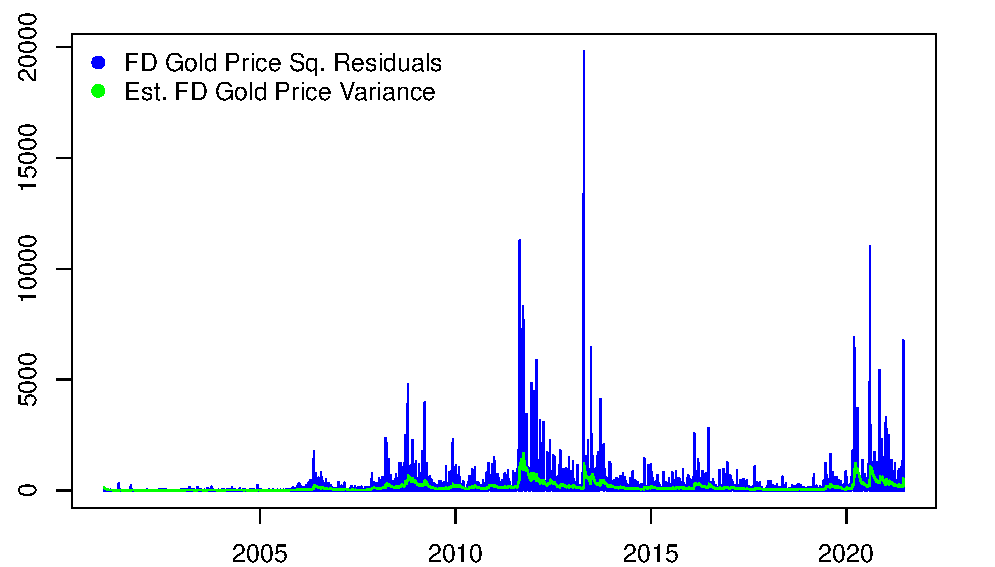
\includegraphics[width=0.90\textwidth]{volatHF}
	\end{figure}	
According to the customary tool AIC, GARCH(1,1), eGARCH(1,1) and iGARCH(1,1) outperform the more standard ARCH(1). In modeling the volatility, we would opt for the simplest, the GARCH(1,1) model, as for this somewhat elementary project this is deemed sufficiently complex. The eGARCH model, however, could be able to give quite reasonable results for prices. Figure 3.4 illustrates how much of the observed volatility can be estimated with our GARCH(1,1) model. Clearly we are unable to properly predict the very large spikes, but we can make reasonable estimations regarding the behavior after such a large spike. This can be easily seen by the periods after the large spike in late 2011 - early 2012. The general shape of the increased volatility is captured but it appears to be scaled down within our model estimation.
\section{Joint Modeling for Gold and Search Interest Index}
\subsection{Exploratory Analysis of the Gold Search Interest Index}
We start by looking a bit closer at the search interest index. A scaled version of this is plotted as the blue line over the entire observational period available in Figure 4.1. We scaled both variables onto a range from zero to one, where we normalize such that the maximum value over the entire time range is one and the minimum value is zero.
	\begin{figure}[!t]
	\centering
	\caption{Relative Gold Price and Gold Search Index from 2004-2021}
	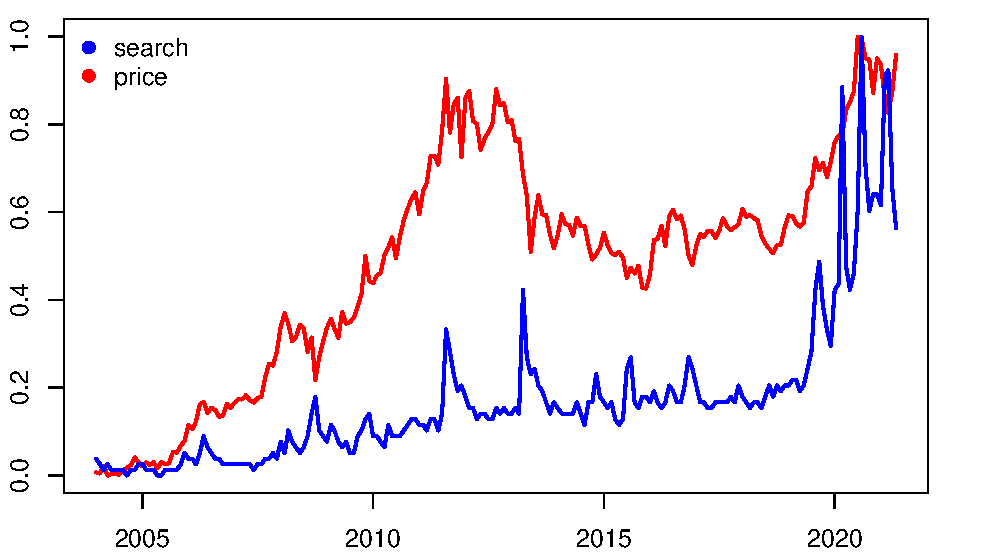
\includegraphics[width=0.90\textwidth]{comparisonPriceSearch}
	\end{figure}
It is easy to see that there was a slight upwards trend in the data over the period from 2004 to 2019. In this period there are two spikes in the data, one around late 2012 and one around late 2013 - early 2014. According to \citeauthor{Desk.24062016} (2016) the first spike appears around the time right before the wedding and festival season in India coinciding with a weak local currency. A similar line of reasoning appears to be the reason for the spike in late 2013 - early 2014. Around late 2019 there appears to be a very strong search interest increase, joint with an increase in volatility. This however is not particularly surprising as gold is often hailed as a good, safe investment in times of increased uncertainty. It is likely that political unrest in India, followed by the start of the Corona crisis are the main drivers for this development. Skepticism about the effects of loosened monetary policy on the value of local currencies in large parts of the world may lead to a flight from local currencies to gold due to its historically stable value. 
%
\subsection{VAR Model for Gold Price and Search Interest Index}
In this section we consider both our variables with a monthly frequency. This means that we need to do the unit-root testing for both variables rather than only the newly introduced one. 

We apply an augmented Dickey-Fuller unit-root test to both variables, where the null is a non-stationary process - namely the random walk with drift and trend components in our test specification:
	\begin{align*}
	 \Delta y_t = a_0 + \gamma \cdot y_{t-1} + a_2 \cdot t + \epsilon_{t}
	\end{align*}
The hypothesis are given by $\tau: \gamma = 0$, $\phi_3: \gamma = a_2 = 0$, and $\phi_2: a_0 = \gamma = a_2 = 0$. For the monthly gold price we have three test-statistics, all three of which fail to reject the null even at a 10\% level. The first of which implies that given the data we cannot reject the hypothesis that the process has a unit-root. From the second it then also follows that we fail to reject the null of a non-zero time-trend term, and from the last one we have that given the data we do not seem to have a non-zero drift term.

Now we consider this same testing procedure for the monthly search index. All three tests reject the null at a 5\% level, the test for $\gamma = 0$ even at the 1\% level. Thus we reject the null of a unit root. Simply from looking at the data we can see that there appears to be some relatively constant trend over time, while same cannot be said for the prices which seem to go down for quite a long period even though there is a strong increase when only looking at the start and end values of the time series. Figure 4.1 illustrates this, again it should be noted that both variables are scaled such that we only look at relative changes for the sake of comparability.

% add description of the model

% add cointegration test and why the model does not work properly

As some of the roots of the characteristic polynomial from the VAR process lie inside of the unit root we do not have a stable process. One possible issue with this modeling might be that we have one I(1) process and one non-stationary process. 
\section{Conclusion}
Given our results from the estimation of the best-prediction model, the ARIMA(0,1,0) model with zero-mean, it appears that our best guess of the next-periods change in daily gold prices is always to assume no changes. This result reminds us of martingale difference sequences, where we have one of the properties given by the expectation at any given time conditional on all past information being zero. However, when adjusting the frequency to a lower value - monthly prices - this is no longer the case. In this case the best-prediction model appears to be a ARIMA(0,1,1) model, i.e.\ a MA(1) model on the first differences. 
%
%
%
%
%
%
%
%
\newpage
\addcontentsline{toc}{section}{References}
\printbibliography
% add google and FRED
\end{document}